\subsection{Verloop van functies}

\subsubsection{Absolute en relatieve extrema}


\begin{definitie}
	Een functie $f$ heeft een \textbf{absoluut maximum} $f(x_{0})$
in het punt $x_{0}\in\textrm{dom}\:f$, als voor alle $x\in\textrm{dom}\:f$
geldt dat $f(x_{0})\geqslant f(x)$

Een functie $f$ heeft een \textbf{absoluut minimum} $f(x_{0})$
in het punt $x_{0}\in\textrm{dom}\:f$, als voor alle $x\in\textrm{dom}\:f$
geldt dat $f(x_{0})\leqslant f(x)$

Een functie $f$ heeft een \textbf{relatief of lokaal maximum}
in het punt $x_{0}$, indien er een open interval $I$ bestaat rond
het punt $x_{0}$ zodat voor alle $x$ in het interval $I$ geldt
dat $f(x_{0})\geqslant f(x)$

Een functie $f$ heeft een \textbf{relatief of lokaal minimum}
in het punt $x_{0}$, indien er een open interval $I$ bestaat rond
het punt $x_{0}$ zodat voor alle $x$ in het interval $I$ geldt
dat $f(x_{0})\leqslant f(x)$

\end{definitie}


\begin{voorbeeld}
\ 	
\gewonefiguur{height=7cm}{2_elem_rekenvaardigheden_B/inputs/verloop_vb1.jpg}
%	\begin{figure}[h]
%\centering{}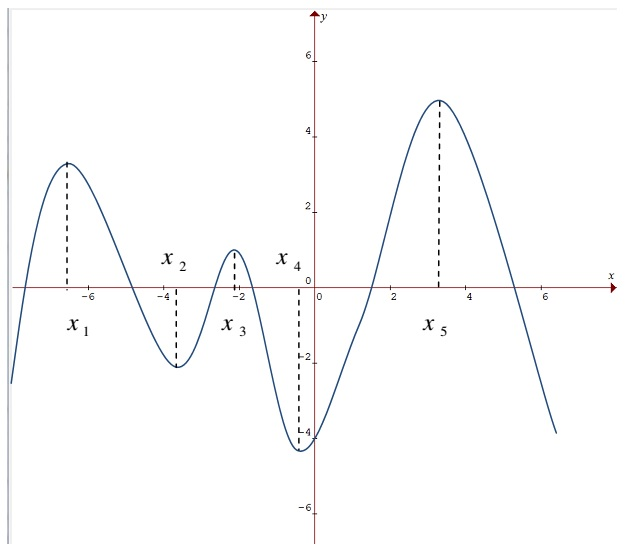
\includegraphics[height=7cm]{2_elem_rekenvaardigheden_B/inputs/verloop_vb1.jpg} 
%\caption{Voorbeeld absolute en relatieve extrema.}
%\label{fig:vb1}
%\end{figure}


Voor de functie in gegeven in bovenstaande figuur zijn $x_{1},\:x_{2},\:x_{3},\:x_{4},\:x_{5}$ relatieve
of lokale extrema. Hiervan zijn $x_{4}$ en $x_{5}$ absolute extrema.

$x_{1},\:x_{3},\:x_{5}$ zijn relatieve of lokale maxima.
Hiervan is $x_{5}$ een absoluut maximum.

$x_{2},\:x_{4}$ zijn relatieve of lokale minima. Hiervan
is $x_{4}$ een absoluut minimum.

\end{voorbeeld}

\subsubsection{Stijgen, dalen en extrema}

De eerste afgeleide speelt een belangrijke rol bij het onderzoek
naar het verloop van een functie. Men zal dus het tekenverloop van
deze afgeleide onderzoeken.




\begin{definitie}
	Als de eerste afgeleide $f^{'}(x)>0$ is in een interval,
dan zal deze functie in dat interval \textbf{stijgen}.

Als de eerste afgeleide $f^{'}(x)<0$ is in een interval,
dan zal deze functie in dat interval \textbf{dalen}.

De functie zal een relatief of lokaal extremum (maximum
of minimum) bereiken waar de kromme overgaat van een stijgende functie
naar een dalende functie of omgekeerd.

Een functie $f(x)$ heeft in het punt $(x_{0},y_{0})$ een
extremum als in dat punt aan de volgende voorwaarden voldaan is:

\begin{itemize}
\item als $f^{'}(x_{0})=0$ en $f^{''}(x_{0})>0$ zal het
extremum een minimum zijn, en
\item als $f^{'}(x_{0})=0$ en $f^{''}(x_{0})<0$ zal het
extremum een maximum zijn.
\end{itemize}

\end{definitie}

\begin{opmerking}
	\ \\
	\begin{itemize}
\item Opmerking 1: in een extremum bezit de functie een horizontale
raaklijn (aangezien $f^{'}(x_{0})=0$ is).
\item Opmerking 2: indien $f^{'}(x_{0})=0$ en ook $f^{''}(x_{0})=0$
werkt deze methode niet om na te gaan of er in $x_{0}$ een extremum
is. In dat geval gaan we naar de derde afgeleide kijken. Als $f^{'''}(x_{0})\neq0$
dan is het punt $x_{0}$ een buigpunt. Indien ook de derde afgeleide
nul is moeten we naar de eerstvolgende afgeleide gaan kijken die niet
nul is. Stel dat deze van de n$^{de}$ orde is, dus $f^{(n)}(x_{0})\neq0$
. Als dan $n$ even is, is er in $x_{0}$ een lokaal minimum als $f^{(n)}(x_{0})>0$
, en een lokaal maximum als $f^{(n)}(x_{0})<0$ . Is de n$^{de}$
oneven dan is $x_{0}$ terug een buigpunt. 

Tip: als je dit moeilijk
kan onthouden, denk dan aan de eenvoudige functies $f(x)=x^{2}$ en
$f(x)=x^{3}$ . De functie $x^{2}$ heeft een minimum in nul, terwijl
$x^{3}$ in de oorsprong een buigpunt heeft.
\end{itemize}

\end{opmerking}



\begin{voorbeeld}
	Onderzoek het stijgen en dalen van volgende functie $f$ met voorschrift: $f(x)=x^{3}-3x^{2}$ in onderstaande figuur.
	
	\gewonefiguur{width=.7\linewidth}{2_elem_rekenvaardigheden_B/inputs/verloop_vb2.jpg}

De eerste afgeleide $f^{'}(x)=3x^{2}-6x$ is nul als $3x^{2}-6x=3x(x-2)=0$, dus als $x=0$ of als $x=2$.

Om de $y$-co\"ordinaat van deze extrema punten te vinden
vullen we $x=0$ en $x=2$ in in de functie $f(x)$. Dit geeft: $f(0)=0$
en $f(2)=-4$.

De functie $f$ zal in de punten $(0,0)$ en $(2,-4)$ een
extremum bezitten. In het punt $(0,0)$ is dit een maximum en in het
punt $(2,-4)$ een minimum. De raaklijn is in die punten ook telkens
horizontaal.

Aangezien de eerste afgeleide een tweedegraadsfunctie is,
zullen we het tekenverloop van de tweedegraadsfunctie toepassen, zie onderstaande tabel.

%\begin{table}
%	\centering
\begin{center}
	\begin{tabular}{c||c|c|c|c|c}
	$x$ &  & 0 &  & 2 & \tabularnewline
	\hline 
	$f^{'}(x)=3x(x-2)$ & + & 0 & - & 0 & + \\
	\hline 
	$f(x)$ &  & 0 &  & -4 & \\
	& $\nearrow$ & max & $\searrow$ & min & $\nearrow$ \\
\end{tabular}
\end{center}

%\caption{Voorbeeld stijgen, dalen en extrema.}
%\label{tab:stijgen}
%\end{table}

%\begin{figure}[h]
%\centering{}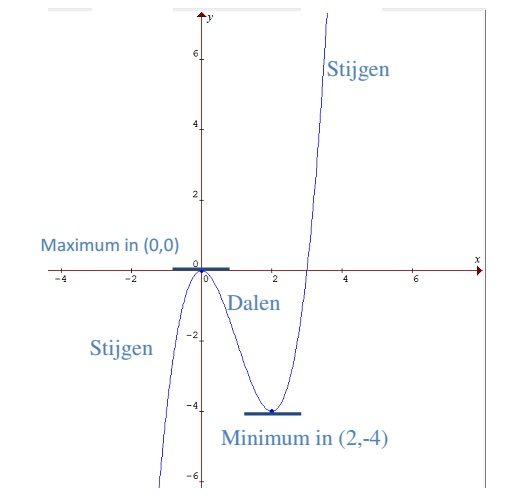
\includegraphics[width=.7\linewidth]{2_elem_rekenvaardigheden_B/inputs/verloop_vb2.jpg}
%\caption{Voorbeeld stijgen en dalen.}
%\label{fig:vb2}
%\end{figure}

\end{voorbeeld}

\subsubsection{Convex, concaaf en buigpunten}

Ook de tweede afgeleide speelt een belangrijke rol bij het
onderzoek naar het verloop van een functie. Men zal dus ook het tekenverloop
van de tweede afgeleide onderzoeken.


\begin{definitie}
	Als de tweede afgeleide $f^{''}(x)>0$ is in een interval,
dan zal de functie in dat interval \textbf{hol of concaaf} zijn (symbool:
$\bigcup$).

Als de tweede afgeleide $f^{''}(x)<0$ is in een interval,
dan zal de functie in dat interval \textbf{bol of convex} zijn (symbool:
$\bigcap$).

Punten waar de kromme overgaat van convex naar concaaf of
omgekeerd, noemt men \textbf{buigpunten}. In een buigpunt verandert
dus de tweede afgeleide van teken. Een functie $f(x)$ heeft in het
punt $(x_{0},y_{0})$ een buigpunt als in dat punt aan de volgende
voorwaarden voldaan zijn: $f^{''}(x_{0})=0$ en $f^{'''}(x_{0})\neq0$

\end{definitie}


\begin{opmerking}
	\ \\
	\begin{itemize}
	\item Opmerking 1: in een buigpunt snijdt de raaklijn de kromme,
	deze raaklijn noemt men de buigraaklijn.
	
	\item Opmerking 2: aangezien de kromming in een buigpunt verandert,
	is een buigpunt nooit een extremum.
\end{itemize}

\end{opmerking}


\begin{voorbeeld}
	Onderzoek het hol en bol zijn van
de functie $f$ met voorschrift $f(x)=x^{3}-3x^{2}$, zie onderstaande figuur.

\gewonefiguur{width=.7\linewidth}{2_elem_rekenvaardigheden_B/inputs/verloop_vb3.jpg}

De eerste afgeleide is $f^{'}(x)=3x^{2}-6x$ 

De tweede afgeleide is $f^{''}(x)=6x-6$ en is nul als $6x-6=6(x-1)=0$
, en dus als $x=1$.

Om de $y$-co\"ordinaat van dit buigpunt te vinden vullen
we $x=1$ in in de functie $f(x)$. Dit geeft: $f(1)=-2$.

Aangezien de tweede afgeleide een eerstegraadsfunctie is,
zullen we het tekenverloop van de eerstegraadsfunctie toepassen, zie onderstaande tabel.

%\begin{table}
%	\centering
\begin{center}
	\begin{tabular}{c||c|c|c}
	$x$ &  & 1 & \tabularnewline
	\hline 
	$f^{''}(x)=6(x-1)$ & - & 0 & +\\
	\hline 
	$f(x)$ & $\bigcap$ & -2 & $\bigcup$\\
	&  & buigpunt & \\
\end{tabular}
\end{center}
%\caption{Voorbeeld convex, concaaf en buigpunten}
%\label{tab:convex}
%\end{table}

\end{voorbeeld}
\begin{voorbeeld}
	Wat kan je zeggen over de functie $f$ met voorschrift
$f(x)=x^{3}$ in het punt waar $x=0$ is?

De eerste afgeleide is $f^{'}(x)=3x^{2}$ en is nul als
$x=0$. Dus $x=0$ kan een extremum zijn.

De tweede afgeleide is $f^{''}(x)=6x$ en is nul als $x=0$.
We kunnen niks zeggen; we moeten naar de eerstvolgende afgeleide gaan
kijken die niet nul is.

De derde afgeleide is $f^{'''}(x)=6$. De derde orde afgeleide
(n=3 is oneven) is niet nul, dus het punt $x=0$ is een buigpunt (en
geen extremum).

\end{voorbeeld}

\begin{voorbeeld}
	Zoek de buigpunten van de functie $f$ met voorschrift
$f(x)=\cos(x)$.

De eerste afgeleide is $f^{'}(x)=-\sin(x)$. De nulpunten
van $\sin x$ zijn $\{x=n\pi\:\textrm{met}\:n\in\mathbb{Z}\}$. In
deze punten kan $f(x)=\cos(x)$ een extremum bereiken.

De tweede afgeleide is $f^{''}(x)=-\cos(x)$. De nulpunten
van $\cos(x)$ zijn $\{x=\frac{\pi}{2}+n\pi\:\textrm{met}\:n\in\mathbb{Z}\}$.
In deze punten verandert de cosinus en dus ook de tweede afgeleide
van teken, dus dit zijn buigpunten. M.a.w. de nulpunten van de functie
$f(x)=\cos(x)$ zijn tevens de buigpunten (dit geldt ook voor de sinus).

\end{voorbeeld}